\documentclass{nsr}

\usepackage{amsmath}
\let\openbox\relax % Avoid a symbol conflict with amsthm.
\usepackage{amsthm}
\usepackage{graphicx}
\usepackage{array}
\usepackage{makecell}
\usepackage{siunitx}
\usepackage{multirow}
\usepackage{booktabs}
\usepackage[table]{xcolor}
\usepackage{algorithm}
\usepackage{hyperref}
\sisetup{
  detect-weight=true,
  detect-inline-weight=math,
  input-symbols = (),
  table-number-alignment = center,
  table-format = 1.4
}

\definecolor{lightgray}{rgb}{0.88,0.88,0.88}

\makeatletter
\def\uns{\ifmmode\,\else$\,$\fi}%

\newtheorem{theorem}{Theorem}
\newtheorem{lemma}{Lemma}
\newtheorem{proposition}{Proposition}
\newtheorem{corollary}{Corollary}
\newtheorem{definition}{Definition}
\newtheorem{remark}{Remark}
\newtheorem{example}{Example}
\makeatother

\jvol{XX}
\jnum{X}
\jyear{Year}
\doi{10.1093/nsr/XXXX}
\received{XX XX Year}
\revised{XX XX Year}
\accepted{XX XX Year}

\markboth{One, Two, and Three}{One, Two, and Three}

\title{An Asynchronous Neuromorphic Architecture for Wearable EEG Emotion Recognition}

\author{Jingxin Liu$^{1,\dagger}$}
\author{Yiming Zhang$^{2,\dagger}$}
\author{Zikai Song$^{1}$}
\author{Zixuan Lai$^{2}$}
\author{Junyi Liu$^{1}$}
\author{Fuze Tian$^{3}$}
\author{Koo Hyoung Lee$^{4}$}
\author{Qunxi Dong$^{1,*}$}
\author{Lixian Zhu$^{1,*}$}
\author{Bin Hu$^{1,*}$}

\affil{$^1$Key Laboratory of Brain Health Intelligent Evaluation and Intervention (Ministry of Education), School of Medical Technology, Beijing Institute of Technology, Beijing 100081, China}
\affil{$^2$Key Laboratory of Brain Health Intelligent Evaluation and Intervention (Ministry of Education), Beijing Institute of Technology, Zhuhai 519088, China}
\affil{$^3$School of Information Science and Engineering, Lanzhou University, Lanzhou 730000, China}
\affil{$^4$NeuroSky, Inc., San Jose, CA 95112, USA}

\authornote{\textbf{Corresponding authors.} E-mail: dongqx@bit.edu.cn
zhulx@bit.edu.cn
bh@bit.edu.cn}

\authornote{Equally contributed to this work}

\begin{document}

\dhead{RESEARCH ARTICLE}
\subhead{INFORMATION SCIENCE}

\abstract[ABSTRACT]{
Neural activity associated with emotion is event driven and temporally sparse, whereas electroencephalography (EEG) is acquired as a continuous signal rather than a usable event stream. Conventional synchronous hardware processes all time steps densely, increasing energy costs during prolonged wearable monitoring. We propose an asynchronous neuromorphic architecture in which a dynamic adaptive spiking neural network converts features derived from EEG into sparse spike events. The model combines a depthwise separable gating module, division-free time-to-first-spike encoding, and adaptive temporal window regulation. The resulting events drive a globally asynchronous, locally synchronous accelerator that activates data movement and computation only for valid events, reducing switching during idle periods. DA-SNN outperforms lightweight models on SEED, SEED-IV, SEED-V, DEAP, and DREAMER. The FPGA implementation achieves an inference latency of $18\,\mu\mathrm{s}$, a dynamic power consumption of $40\,\mathrm{mW}$, and a total energy consumption of $2.66\,\mu\mathrm{J}$ per inference.
}

%\jelcode{Pa, J6, P16, E22}

\keywords{
affective electroencephalography, asynchronous neuromorphic architecture, spiking neural network, globally asynchronous locally synchronous, wearable monitoring}


\maketitle


\section{INTRODUCTION}\label{sec1}
Emotions shape perception and decision making \cite{ref73}, while systems that respond to affect are increasingly studied in human--robot interaction, brain--computer interfaces (BCIs), and healthcare \cite{ref1,ref3,ref4,ref12}. Among physiological modalities, electroencephalography (EEG) provides direct access to central nervous system dynamics at high temporal resolution \cite{ref5,ref74}. Sparse neural coding and spike communication motivate event-driven representations that avoid treating all activity as uniformly dense \cite{ref28,ref75}.

Recent progress in wearable EEG devices has lowered the hardware barrier to prolonged monitoring. Lightweight sensors \cite{ref9}, hydrogel epidermal electrodes \cite{ref10}, and stable analog front-end circuits \cite{ref11} support prolonged EEG recording outside conventional laboratory systems. Signal acquisition alone, however, is insufficient for wearable emotion recognition. In unconstrained environments, emotions are continuous, slowly varying, and strongly subject dependent \cite{ref12}. The inference system must therefore operate under constraints on power, intrusiveness, and monitoring duration \cite{ref13}.

Convolutional neural networks (CNNs) have been widely adopted in emotion recognition and BCI tasks \cite{ref18}. For example, EEGNet \cite{ref56} processes continuously sampled EEG signals within fixed analysis windows to learn temporal dynamics and spatial patterns. Its computational cost is closely coupled to the input sampling rate, so the overhead scales with analysis duration during prolonged monitoring. Long short-term memory (LSTM) models \cite{ref20,ref21} offer another approach to EEG time series analysis through recursive updates of hidden states. These temporal dependencies constrain parallel execution across recurrent steps and complicate efficient hardware acceleration \cite{ref76}. Computation latency therefore grows with sequence length, limiting real time performance and energy efficiency. Graph convolutional network (GCN) methods, such as MSFR-GCN \cite{ref22}, instead model the spatial topology among electrodes. Multiscale spatial modeling and node interactions improve the representation of complex correlations across electrodes \cite{ref23,ref24}. This expressiveness comes with substantial overhead from graph aggregation and irregular access patterns, which stress the memory hierarchy.

Overall, synchronous acquisition followed by dense computation couples computational cost to the input sampling rate, increasing power and latency as monitoring duration grows. Neural activity motivates event representations because it is distributed and temporally structured, but scalp EEG is acquired as a continuously sampled waveform. Realizing an engineering benefit requires the model to convert features derived from EEG into sparse events that suppress unnecessary data movement and hardware state updates.

Model compression techniques such as pruning, quantization, and knowledge distillation reduce arithmetic cost \cite{ref25,ref26,ref77}, but dense execution can still update globally clocked datapaths at every processed time step. This residual cost is relevant to wearable EEG emotion recognition, where power and response time are constrained.

Sparse spikes yield hardware savings only when datapaths and memory transfers respond to event validity. Continuously active hardware can otherwise erode the advantage of algorithmic sparsity. This requirement motivates the integrated design of event encoding, transfer between clock domains, spiking computation, and classification readout.

\begin{figure*}[t]
\centering
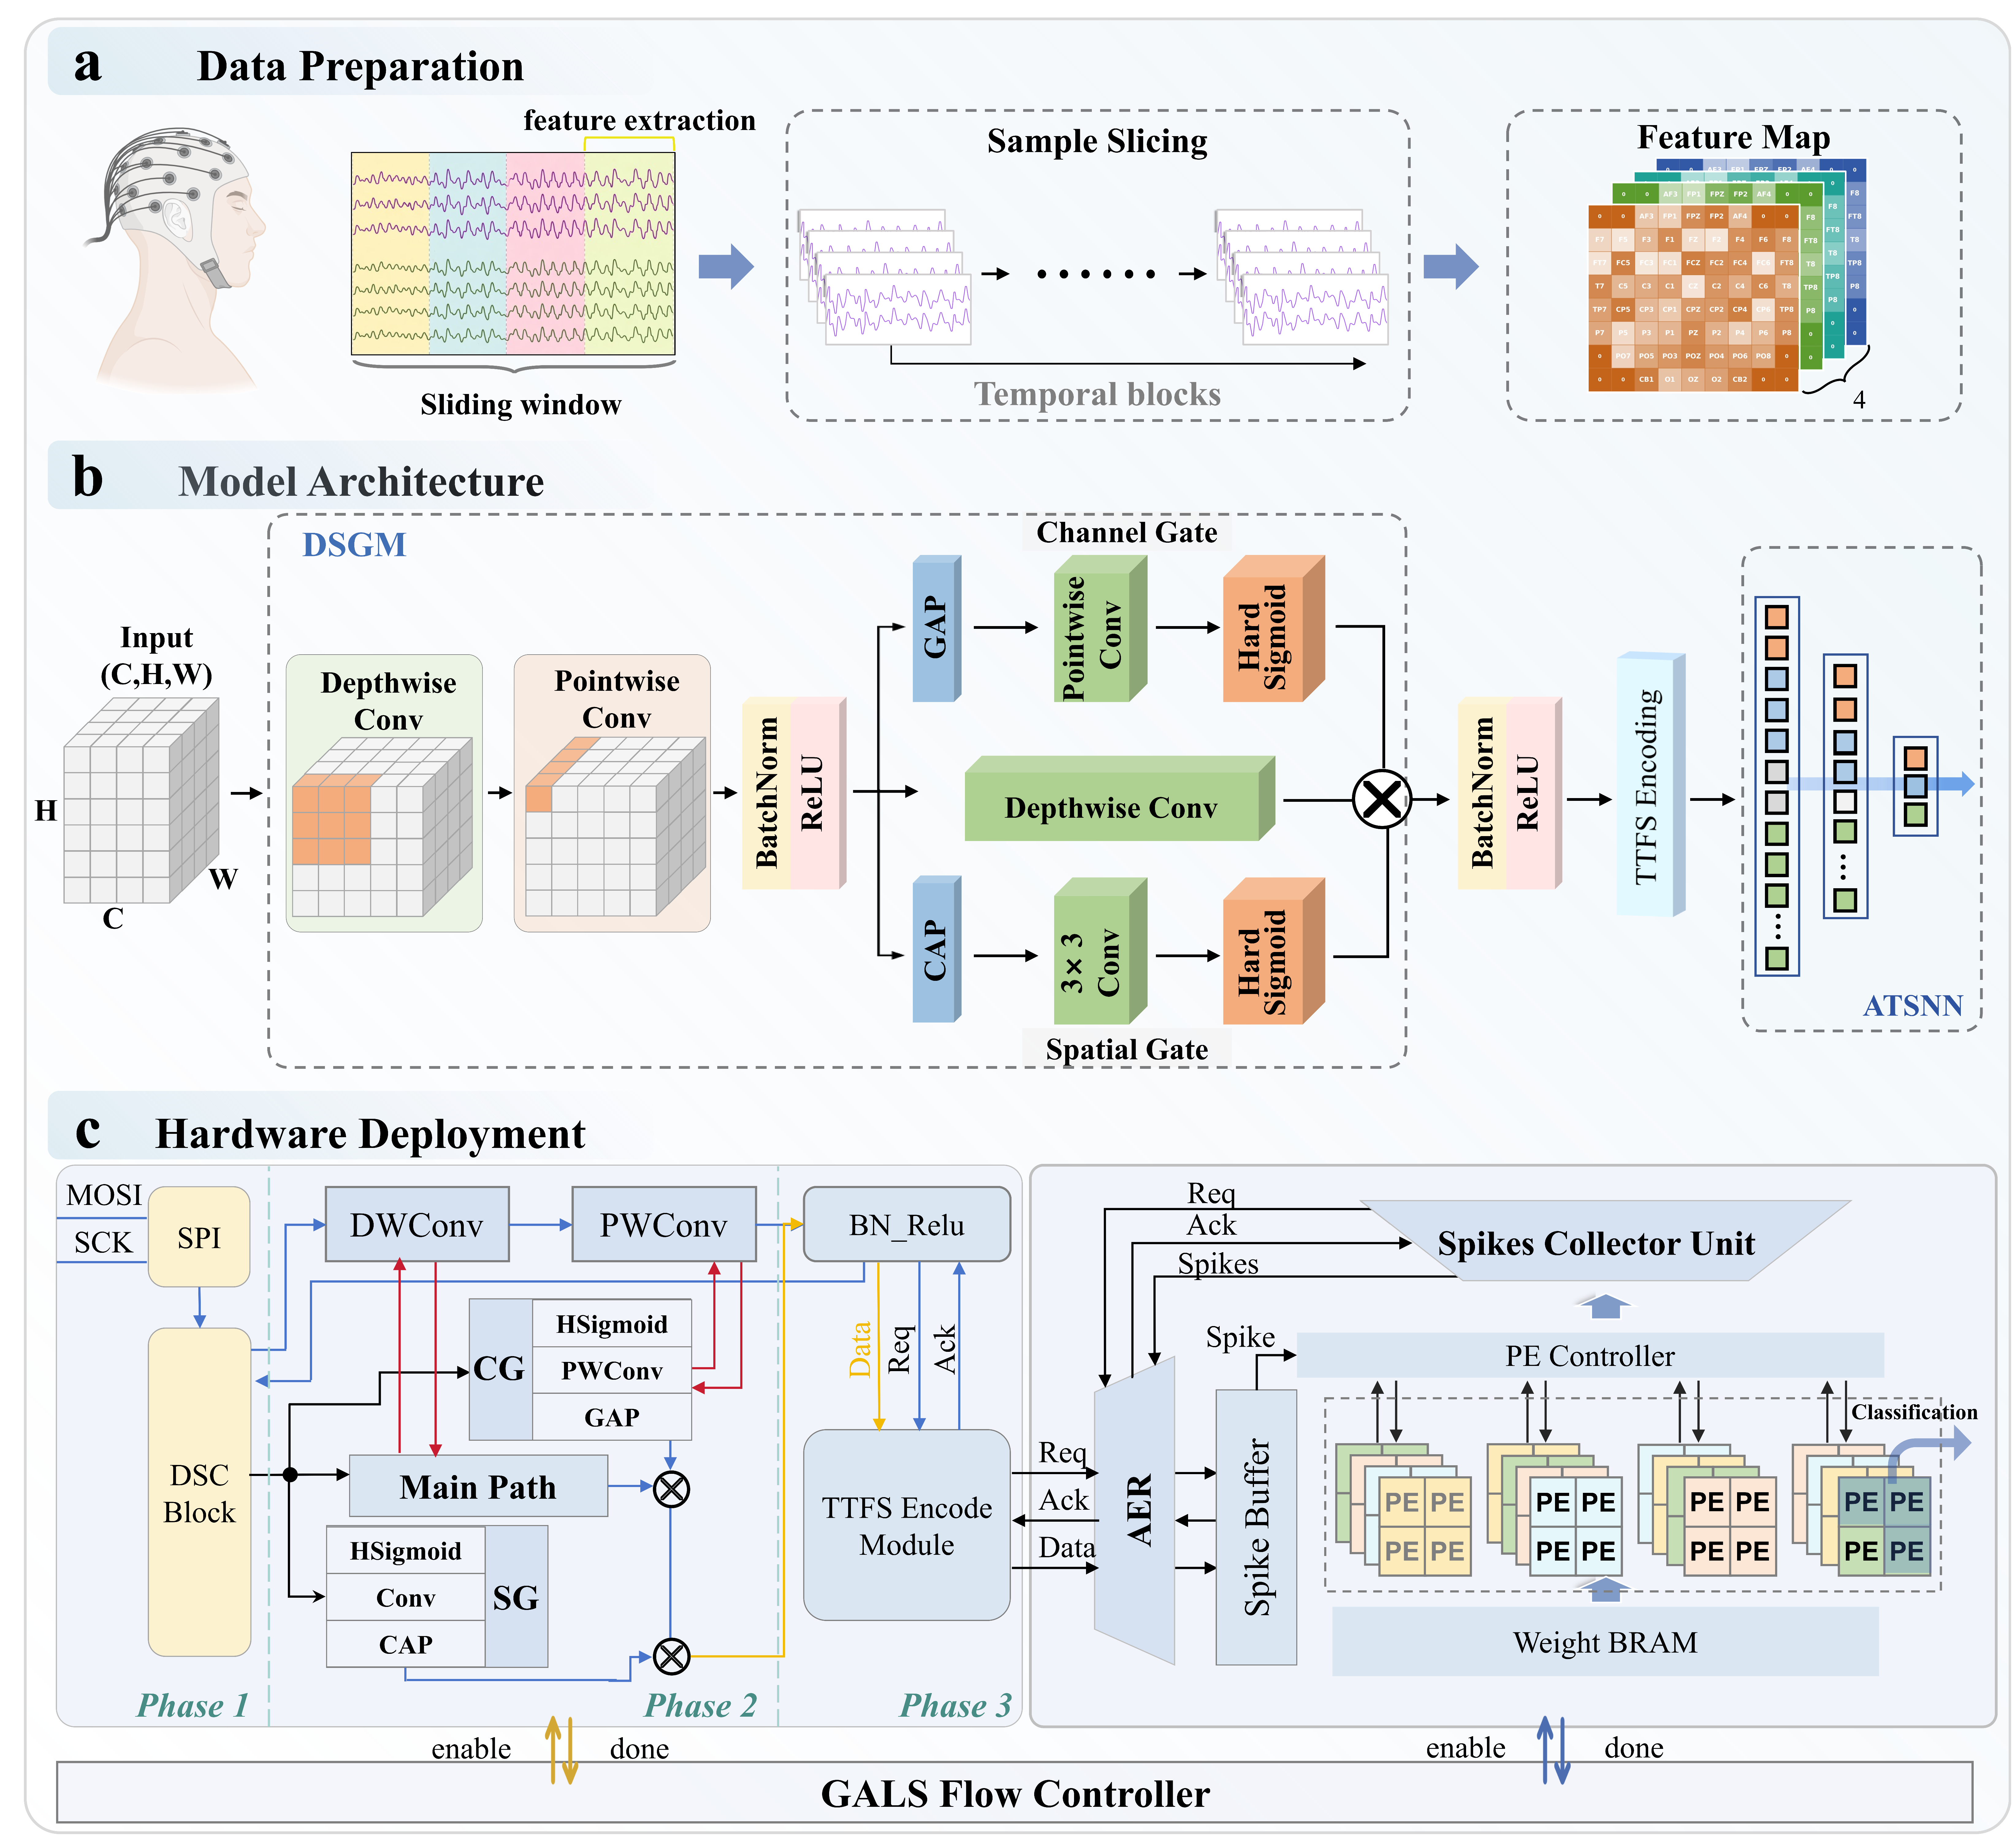
\includegraphics[width=0.95\textwidth]{figures/Overview.eps}
\caption{\textbf{Jointly optimized neuromorphic architecture for globally asynchronous, locally synchronous (GALS) event-driven inference.}
EEG signals are transformed into spatial-spectral representations and processed by a lightweight dynamic adaptive spiking neural network model with depthwise separable convolution.
Dense activations are encoded into sparse spike times via division-free time-to-first-spike and transferred as address-event representation (AER) packets for event-triggered accelerator inference.
A GALS architecture is adopted at the system level to coordinate event-driven operation between independent locally synchronous clock islands.}
\label{fig:system_overview}
\end{figure*}
{\small\noindent\textbf{Alt text:} A system overview links continuous EEG preprocessing to event-driven inference. EEG recordings are converted into spatial--spectral tensors. DA-SNN refines the dense features and encodes them as sparse spike times. A GALS accelerator transfers address and timestamp events between locally synchronous domains for emotion classification.\par}
Spiking neural networks (SNNs) offer a biologically inspired, event-driven alternative to conventional artificial neural networks (ANNs) \cite{ref27}. Because SNN neurons emit spikes only when their membrane potential crosses a threshold, sparse activity can reduce computation and memory traffic \cite{ref28}. Previous studies have reported SNN EEG decoding and emotion classification on neuromorphic processors and constrained wearable hardware \cite{ref31,ref32,ref33}. Kumar et al. \cite{ref31}, for example, implemented an SNN EEG decoder on neuromorphic processors to improve energy efficiency. Recurrent SNNs can also model the temporal evolution of EEG signals \cite{ref32}, while simplified spiking dynamics enable depression recognition on microcontrollers \cite{ref33}. Wearable hardware benefits when execution and data movement respond directly to sparse model activity. In synchronous CMOS systems, unnecessary clocked switching remains a major source of dynamic power \cite{ref78}. Continuously active datapaths can therefore retain clocked state updates and memory activity despite sparse spikes. We couple an EEG SNN with a GALS substrate that transfers sparse events between locally synchronous domains and activates only the required paths.

We therefore propose an integrated neuromorphic architecture for edge EEG inference. Its Dynamic Adaptive Spiking Neural Network (DA-SNN) uses a lightweight depthwise separable gating module (DSGM) to separate spatial and channel saliency and reduce spatiotemporal redundancy. Division-free time-to-first-spike (DF-TTFS) encoding and adaptive temporal window regulation then convert model activity into events suitable for hardware. DF-TTFS removes floating-point division from the critical inference path. The sparse event streams drive a custom globally asynchronous, locally synchronous (GALS) accelerator \cite{ref69}. Two local clock islands exchange address and timestamp events through a bundled-data request/acknowledgment (Req/Ack) interface. Local clock enables suppress unnecessary state updates in idle modules. Together, these elements map tensors derived from EEG to sparse events and GALS execution. We report model and FPGA performance within explicit protocol and measurement boundaries that include interface cost and both dynamic and static power.


\begin{figure*}[t]
\hspace*{-2.8cm}
\begin{minipage}{\dimexpr\textwidth+2.8cm\relax}
\centering
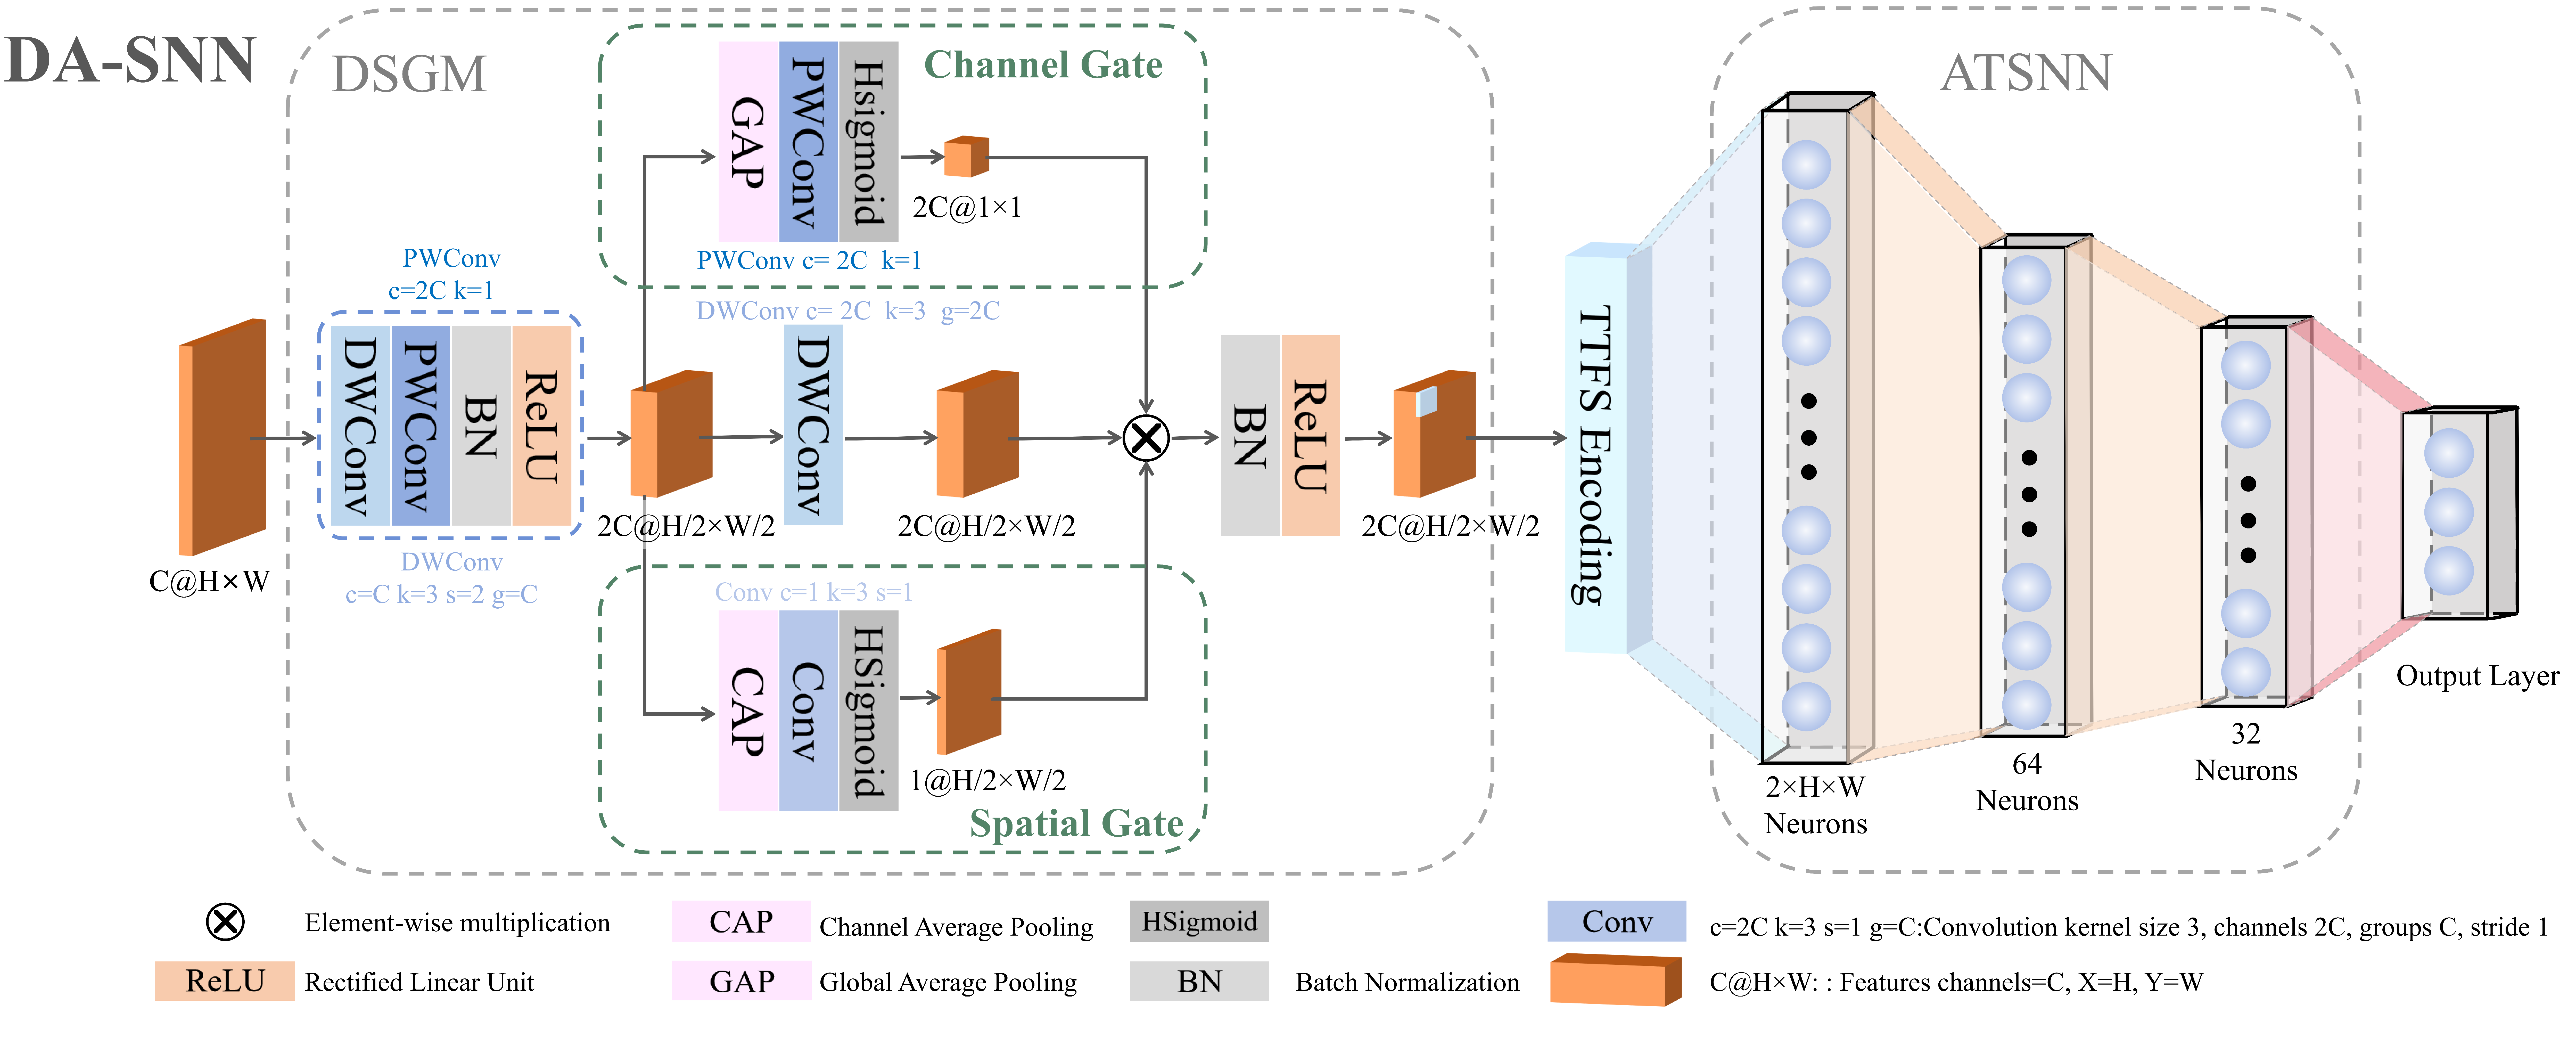
\includegraphics[width=\textwidth]{figures/DA-SNN.eps}
\caption{\textbf{The proposed DA-SNN model framework.}
The input is a dense tensor derived from EEG. Its feature channel axis contains temporally contiguous power spectral entropy maps, and its two spatial axes represent the topographic electrode grid. DSGM combines depthwise separable feature extraction with channel and spatial gating. The circled multiplication mark denotes elementwise multiplication, corresponding to the Hadamard product used in the main text. In labels of the form $C@H\times W$, the at sign separates the number of feature channels from the spatial height and width. DWConv, depthwise convolution; PWConv, pointwise convolution; GAP, global average pooling; CAP, channel average pooling; BN, batch normalization; HSigmoid, Hard-Sigmoid; DF-TTFS, division-free time-to-first-spike; ATSNN, adaptive temporal spiking neural network. DF-TTFS preserves the tensor shape while converting the DSGM output into spike times before ATSNN classification. Labels showing half spatial size are schematic. The Supplementary Information provides the exact dimensions, convolution parameters, and broadcasting rules for each dataset.}
{\small\noindent\textbf{Alt text:} A schematic of DA-SNN from left to right. A topographic tensor derived from EEG passes through depthwise separable feature extraction and parallel channel, spatial, and main feature paths. Their outputs are combined by elementwise multiplication. The resulting dense feature tensor is converted to spike times and processed by successive spiking layers to produce the emotion class.\par}
\label{fig:DA-SNN}
\end{minipage}
\end{figure*}

\section{RESULTS}
We evaluate DA-SNN and its GALS hardware architecture at the model and implementation levels. The results first define the neuromorphic framework and spiking dynamics, then compare classification performance across five EEG benchmarks. Subsequent analyses examine sensitivity to controlled perturbations and weight quantization, model-level efficiency, and the field-programmable gate array (FPGA) implementation.


\subsection{Neuromorphic framework for EEG emotion recognition}

The proposed framework for wearable EEG emotion recognition integrates data preprocessing, model architecture, and hardware deployment (Fig.~\ref{fig:system_overview}). Continuous EEG recordings are first z-score normalized and divided into outer windows without overlap. Within each outer window, power spectral entropy (PSE) is calculated over $N_f$ temporally contiguous bins. The electrode values in each bin are projected onto an $H\times W$ topographic grid and stacked to form a dense tensor in $\mathbb{R}^{N_f\times H\times W}$. Thus, the input feature channel axis represents consecutive PSE maps, whereas EEG electrodes occupy positions on the two spatial axes. The Supplementary Information describes LDS smoothing within each trial and provides complete tensor definitions for every dataset.

The model then maps this dense EEG-derived tensor to a sparse spike-time representation. As shown in Fig.~\ref{fig:DA-SNN}, DA-SNN processes the tensor through DSGM for gated feature extraction, division-free TTFS encoding \cite{TTFS}, and an adaptive temporal spiking neural network (ATSNN) for classification. DSGM operates on dense-valued feature tensors; DF-TTFS defines the tensor-to-event boundary by mapping refined activations to spike times before spiking inference.

The DSGM module combines depthwise separable convolution with parallel channel and spatial gating. Given an input feature map $X \in \mathbb{R}^{C\times H\times W}$, the initial depthwise and pointwise convolutions produce an aligned feature tensor $U\in\mathbb{R}^{C_o\times H'\times W'}$, and a second depthwise convolution forms the main feature path:
\begin{equation}
\begin{aligned}
U &= f_{\mathrm{PW}}\!\bigl(f_{\mathrm{DW}}(X)\bigr),\\
F_{\mathrm{main}} &= f_{\mathrm{main}}(U),
\end{aligned}
\label{eq:dsgm_backbone}
\end{equation}
where $f_{\mathrm{DW}}(\cdot)$ and $f_{\mathrm{PW}}(\cdot)$ denote the stride-2 depthwise and pointwise feature transformations, respectively, and $f_{\mathrm{main}}(\cdot)$ denotes the stride-1 depthwise convolution on the main path. For the first network input, $C=N_f$ is the number of stacked PSE temporal-bin maps, whereas EEG electrodes occupy positions on the $H\times W$ grid. The channel gate operates on $U$ and aggregates its spatial axes to form $s\in\mathbb{R}^{C_o\times1\times1}$ and weights $G_{\mathrm{ch}}\in\mathbb{R}^{C_o\times1\times1}$:
\begin{equation}
\left\{
\begin{aligned}
s_c &= \frac{1}{H'W'}\sum_{i=1}^{H'}\sum_{j=1}^{W'}U_{c,i,j},\quad c=1,\dots,C_o,\\[0.5mm]
\sigma(x) &= \mathrm{clip}\!\left(\frac{x}{8}+0.5,\,0,\,1\right)\\[0.5mm]
G_{\mathrm{ch}} &= \sigma\!\left(f_{\mathrm{conv}}^{1\times1}(s_c)+b_{\mathrm{ch}}\right)
\end{aligned}
\right.,
\label{eq:dsgm_ch_gate}
\end{equation}
where $b_{\mathrm{ch}}$ is the bias and $\sigma(\cdot)$ is the Hard-Sigmoid function. The spatial gate averages $U$ over its feature channel axis, yielding a descriptor $S_{\mathrm{sp}}\in\mathbb{R}^{1\times H'\times W'}$ and spatial weights $G_{\mathrm{sp}}\in\mathbb{R}^{1\times H'\times W'}$:
\begin{equation}
\left\{
\begin{aligned}
S_{\mathrm{sp}} &= \frac{1}{C_o}\sum_{c=1}^{C_o}U_c,\\[0.5mm]
G_{\mathrm{sp}} &= \sigma\!\left(f_{\mathrm{conv}}^{3\times3}(S_{\mathrm{sp}})+b_{\mathrm{sp}}\right)
\end{aligned}
\right.,
\label{eq:dsgm_sp_gate}
\end{equation}
where $b_{\mathrm{sp}}$ is the bias. The aligned main-path features are modulated by the two gates, followed by batch normalization and ReLU activation:
\begin{equation}
F_{\mathrm{out}} = f_{\mathrm{ReLU}}\!\Bigl(f_{\mathrm{BN}}\bigl(F_{\mathrm{main}}\odot G_{\mathrm{ch}}\odot G_{\mathrm{sp}}\bigr)\Bigr),
\label{eq:dsgm_out}
\end{equation}
where $\odot$ denotes elementwise multiplication. At fusion, the channel gate is broadcast over the two spatial axes and the spatial gate over the feature channel axis. All three tensors therefore share the $C_o\times H'\times W'$ feature resolution. The Supplementary Information provides the complete kernel, stride, padding, grouping, shape, and broadcasting specifications for every dataset.

\begin{table*}[t]
\centering
\hspace*{-2.8cm}
\begin{minipage}{1.2\textwidth}
\caption{Subject-dependent performance under a random window-level 80/20 evaluation protocol (Acc, accuracy; F1, macro-F1; Spe, macro-specificity).}
\label{tab:overall_15models}
\setlength{\tabcolsep}{2.5pt}
\renewcommand{\arraystretch}{1.3}
\footnotesize
\resizebox{\textwidth}{!}{%
\begin{tabular}{l*{15}{c}}
\toprule
\multirow{2}{*}{Method}
& \multicolumn{3}{c}{SEED}
& \multicolumn{3}{c}{SEED-IV}
& \multicolumn{3}{c}{SEED-V}
& \multicolumn{3}{c}{DEAP}
& \multicolumn{3}{c}{DREAMER} \\
\cmidrule(lr){2-4}\cmidrule(lr){5-7}\cmidrule(lr){8-10}\cmidrule(lr){11-13}\cmidrule(lr){14-16}
& {Acc (\%)} & {F1 (\%)} & {Spe (\%)}
& {Acc (\%)} & {F1 (\%)} & {Spe (\%)}
& {Acc (\%)} & {F1 (\%)} & {Spe (\%)}
& {Acc (\%)} & {F1 (\%)} & {Spe (\%)}
& {Acc (\%)} & {F1 (\%)} & {Spe (\%)} \\
\midrule
RF\cite{ref52} & 91.91 & 91.65 & 93.30 & 89.85 & 87.86 & 92.30 & 89.23 & 87.82 & 91.98 & 79.43 & 76.31 & 92.58 & 86.14 & 81.34 & 92.22 \\
k-NN\cite{ref53} & 90.82 & 89.90 & 92.12 & 89.05 & 87.71 & 92.26 & 87.91 & 87.24 & 91.27 & 82.75 & 79.86 & 90.20 & 88.88 & 88.02 & 91.89 \\
XGBoost\cite{ref54} & 88.11 & 86.60 & 90.72 & 86.27 & 85.37 & 91.35 & 88.41 & 85.20 & 92.30 & 75.26 & 75.47 & 91.21 & 85.56 & 85.46 & 89.95 \\
SqueezeNet\cite{ref57} & 94.04 & 93.31 & 96.58 & 92.35 & 92.63 & 97.44 & 90.37 & 91.29 & 97.68 & 67.74 & 73.00 & 85.38 & 91.08 & 90.17 & 96.64 \\
MobileNetV3-Small\cite{ref58} & 93.40 & 90.14 & 94.23 & 92.61 & 93.52 & 97.51 & 91.91 & 91.66 & 94.66 & 84.11 & 82.92 & 94.53 & 89.24 & 89.21 & 96.29 \\
MobileNetV3-Large\cite{ref58} & 90.85 & 91.76 & 92.66 & 90.34 & 88.88 & 94.87 & 89.73 & 88.36 & 88.94 & 86.29 & 82.59 & 92.17 & 91.63 & 91.37 & \textbf{97.62} \\
ShuffleNetV2\cite{ref59} & 91.01 & 92.43 & 95.51 & 93.71 & 92.61 & 97.91 & 90.22 & 91.22 & 95.47 & 77.21 & 77.17 & 92.02 & 92.85 & \textbf{92.88} & 97.49 \\
EfficientNet-B0\cite{ref60} & 95.35 & 94.60 & 97.67 & 92.16 & 92.34 & 97.34 & 91.65 & 93.34 & 97.58 & 83.92 & 83.90 & 94.43 & 88.35 & 87.54 & 94.04 \\
EfficientNet-B3\cite{ref60} & 96.03 & 95.58 & 98.02 & 92.96 & 93.58 & 97.60 & 91.19 & 91.35 & 96.96 & 70.14 & 72.71 & 89.35 & 85.54 & 86.09 & 92.56 \\
Deep ConvNet\cite{ref55} & 95.88 & 94.91 & 97.93 & 92.48 & 92.06 & 97.46 & 90.51 & 89.58 & 97.63 & 82.19 & 84.10 & 89.99 & 89.81 & 90.53 & 94.95 \\
Shallow ConvNet\cite{ref55} & 92.27 & 94.18 & 96.15 & 89.49 & 90.32 & 96.12 & 85.78 & 87.69 & 96.20 & 80.58 & 79.85 & 89.79 & 83.61 & 82.80 & 86.28 \\
EEGNet\cite{ref56} & 91.34 & 91.89 & 95.67 & 88.03 & 83.46 & 90.99 & 86.08 & 85.65 & 93.89 & 81.75 & 80.18 & 91.02 & 86.45 & 85.97 & 88.19 \\
EESCN\cite{ref61} & 96.08 & 94.85 & 98.04 & 92.60 & 92.54 & 97.15 & 89.01 & 90.15 & 95.91 & 87.65 & 86.55 & 94.82 & 92.32 & 91.84 & 97.27 \\
DH-SNN\cite{ref62} & 96.54 & 95.75 & \textbf{98.40} & 93.08 & 91.44 & 98.27 & 91.51 & \textbf{94.42} & 97.16 & 75.75 & 78.24 & 88.85 & 89.89 & 90.78 & 96.59 \\
\textbf{DA-SNN} & $\mathbf{96.85 \pm 1.44}$ & $\mathbf{96.81 \pm 0.92}$ & $97.08 \pm 0.87$ & $\mathbf{93.87 \pm 5.99}$ & $\mathbf{94.10 \pm 5.30}$ & $\mathbf{98.35 \pm 3.59}$ & $\mathbf{92.10 \pm 6.33}$ & $93.31 \pm 5.77$ & $\mathbf{97.72 \pm 3.89}$ & $\mathbf{87.96 \pm 5.44}$ & $\mathbf{86.83 \pm 8.53}$ & $\mathbf{97.62 \pm 3.20}$ & $\mathbf{94.18 \pm 2.20}$ & $91.73 \pm 2.56$ & $94.38 \pm 4.64$ \\
\bottomrule
\end{tabular}
}
\vspace{2pt}

\footnotesize\textit{Note:} The split unit is the outer window; subjects and trials may occur in both training and held-out evaluation partitions. Accuracy is window-level accuracy, macro-F1 is the unweighted mean of per-class F1, and macro-specificity is the unweighted mean of one-versus-rest specificity. DA-SNN values are mean $\pm$ sample standard deviation across repeated runs; baseline point estimates are shown as available. Bold metric values indicate the best result for each dataset and metric. Full preprocessing, split, checkpoint-selection, and aggregation details are provided in the Supplementary Methods.
\end{minipage}
\end{table*}

Conventional neuron models such as Leaky Integrate-and-Fire (LIF) \cite{ref79} require recurrent membrane updates and decay operations. ATSNN instead adopts the B1 model of Stanojevi\'{c} et~al. \cite{ref46} as its spike time substrate. This prior model provides piecewise linear dynamics with a constant slope, a single spike representation, and cascaded temporal windows across layers. We adapt its temporal window regulation to the EEG focused DA-SNN pipeline. For layer $n$, the half-open window is $[T_{\min}^{(n)},T_{\max}^{(n)})$, with $T_{\min}^{(n)}=T_{\max}^{(n-1)}$. The membrane potential $V_i^{(n)}(t)$ of neuron $i$ is governed by
\begin{equation}
\label{eq:b1_dynamics}
\epsilon \frac{dV_i^{(n)}}{dt} =
\begin{cases}
\displaystyle \sum\nolimits_j W_{ij}^{(n)} H\!\left(t-T_j^{(n-1)}\right), & t < T_{\min}^{(n)},\\[0.4em]
1, & T_{\min}^{(n)} \le t < T_{\max}^{(n)}
\end{cases},
\end{equation}
Here $j$ indexes presynaptic neurons, $W_{ij}^{(n)}$ is the synaptic weight, $T_j^{(n-1)}$ is the presynaptic spike time, and $H(\cdot)$ is the Heaviside function. The firing threshold $\vartheta_i^{(n)}$ is expressed in normalized membrane-potential units, while $\epsilon>0$ converts the threshold term into a temporal offset. Integrating Eq.~(\ref{eq:b1_dynamics}) gives the theoretical threshold-crossing time $\tilde{T}_i^{(n)}$; an explicit timeout rule then determines whether this crossing is an active spike:
\begin{equation}
\label{eq:b1_combined}
\left\{
\begin{aligned}
\tilde{T}_i^{(n)} &= T_{\min}^{(n)} + \epsilon \vartheta_i^{(n)} + \sum\nolimits_j W_{ij}^{(n)}\!\left(T_j^{(n-1)} - T_{\min}^{(n)}\right), \\
M_i^{(n)} &= \mathbf{1}\!\left[\tilde{T}_i^{(n)} < T_{\max}^{(n)}\right], \\
T_i^{(n)} &= M_i^{(n)}\tilde{T}_i^{(n)} + \left(1-M_i^{(n)}\right)T_{\max}^{(n)}
\end{aligned}
\right.,
\end{equation}
The first line is the closed form threshold crossing time, whereas the latter two lines define censoring at the upper boundary. The strict inequality makes a crossing at $T_{\max}^{(n)}$ inactive. Thus, $T_i^{(n)}=T_{\max}^{(n)}$ is a numerical placeholder whose validity is determined by $M_i^{(n)}$. Because the next layer starts at this boundary, a censored placeholder contributes zero temporal offset. Under the original B1 identity parameterization ($A_i^{(n)}=0$ and $B_i^{(n)}=1$) and its associated mapping assumptions, spike latency corresponds exactly to a ReLU activation. This property makes the B1 model suitable for hardware. DA-SNN extends this substrate with EEG specific DSGM processing, power-of-two DF-TTFS encoding, temporal regulation referenced to the midpoint, and integrated GALS acceleration.

Continuous DSGM features are converted into sparse spike times for the downstream ATSNN using TTFS coding, which maps stronger activations to earlier spikes. Standard TTFS normalizes input activation $V_{\mathrm{in}}$ by division as
\begin{equation}
V_{\mathrm{norm}} = \frac{V_{\mathrm{in}} - V_{\min}}{V_{\max} - V_{\min}},
\label{eq:standard_ttfs}
\end{equation}
where $V_{\min}$ and $V_{\max}$ denote the minimum and maximum bounds. We instead implement a DF-TTFS encoder that adapts to the dynamic range. The complete encoding is
\begin{equation}
\left\{
\begin{aligned}
S_p &= 2^{\left\lceil \log_2\!\left(\max\!\left(V_{\max}-V_{\min},\delta\right)\right) \right\rceil}, \qquad \delta>0, \\
V_{\mathrm{norm}} &= \mathrm{clip}\left(\frac{V_{\mathrm{in}}-V_{\min}}{S_p}, 0, 1\right) \\
T_{\mathrm{spike}} &= T_{\max} - \mathrm{round}\left(V_{\mathrm{norm}} (T_{\max}-T_{\min})\right)
\end{aligned}
\right.,
\label{eq:ttfs_div_free}
\end{equation}
where $S_p$ is the power-of-two scaling factor, $\delta$ is a positive numerical safeguard for a zero or near-zero activation range, $\mathrm{clip}(\cdot)$ clamps values to $[0,1]$, and $T_{\mathrm{spike}}$ is the discrete spike time.

For an active neuron, the local weight gradient contains a temporal offset from the presynaptic neuron:
\begin{equation}
\frac{\partial \mathcal{L}}{\partial W_{ij}^{(n)}} = \frac{\partial \mathcal{L}}{\partial T_i^{(n)}} \cdot \left(T_j^{(n-1)} - T_{\min}^{(n)}\right).
\label{eq:grad_w}
\end{equation}
This local relation motivates regulating the range of presynaptic spike times. ATSNN monitors the earliest valid spike time $T_{e}^{(n)}$ in layer $n$ and updates the upper bound of the temporal window as
\begin{equation}
T_{\max}^{(n)\prime} = T_{\max}^{(n)} + \lambda\!\left(T_{e}^{(n)} - \frac{T_{\max}^{(n)} + T_{\min}^{(n)}}{2}\right),
\label{eq:atsnn_update}
\end{equation}
where $\lambda$ controls the adaptation rate. Stanojevi\'{c} et~al. also adapt the upper window boundary during training through a conditional rule centered on that boundary. Equation~(\ref{eq:atsnn_update}) uses the signed displacement of the earliest valid spike from the window midpoint. The window can therefore contract for early activity or expand for late activity. The updated bound propagates to the next layer through $T_{\min}^{(n+1)}=T_{\max}^{(n)\prime}$; when no valid spike is observed, the boundary remains unchanged (Supplementary Note~S2.3).

The output layer is a continuous, nonspiking integrator. With the cascade condition $T_{\min}^{(L)}=T_{\max}^{(L-1)}$, an inactive hidden neuron has $T_j^{(L-1)}=T_{\min}^{(L)}$ and therefore contributes zero. The class-$k$ logit can consequently be written in equivalent observed-time and explicitly masked forms:
\begin{equation}
\begin{aligned}
z_k
&= \sum\nolimits_j W_{kj}^{(L)}\!\left(T_{\min}^{(L)} - T_j^{(L-1)}\right) + \epsilon \vartheta_k^{(L)} \\
&= \sum\nolimits_j W_{kj}^{(L)} M_j^{(L-1)}\!\left(T_{\min}^{(L)} - \tilde{T}_j^{(L-1)}\right) + \epsilon \vartheta_k^{(L)}.
\end{aligned}
\label{eq:out_logit}
\end{equation}
Thus, the active mask identifies a censored $T_{\max}$ value as a boundary placeholder. The network predicts the class with the highest logit.


\subsection{Emotion Recognition Performance Across EEG Benchmarks}

Main Table~\ref{tab:overall_15models} reports the subject-dependent benchmark on five standard EEG emotion recognition datasets using a random window-level 80/20 split. This setting enables comparison of 15 models under a common protocol. Complementary subject-independent evaluations use leave-one-subject-out (LOSO) for SEED, SEED-IV, and SEED-V, and five fixed subject holdout splits for DEAP and DREAMER. These evaluations are described in the Supplementary Methods and reported in Supplementary Tables~S4 and S5. The two settings address different objectives, so their absolute values require separate interpretation.

DA-SNN achieves the highest accuracy on all five subject-dependent benchmarks (Table~\ref{tab:overall_15models}): $96.85 \pm 1.44\%$ on SEED, $93.87 \pm 5.99\%$ on SEED-IV, $92.10 \pm 6.33\%$ on SEED-V, $87.96 \pm 5.44\%$ on DEAP, and $94.18 \pm 2.20\%$ on DREAMER. This advantage spans categorical emotion tasks with three to five classes and the valence--arousal tasks in DEAP and DREAMER. Macro-F1 and macro-specificity are also competitive, but leadership in these metrics varies across datasets. The cross-dataset performance claim therefore concerns accuracy, which is consistently highest, rather than every reported metric.

Ablations across datasets further separate the roles of the principal components (Supplementary Table~S6). Across five random seeds, replacing the adaptive temporal window with fixed windows reduces mean accuracy by 4.98, 10.75, and 0.83 percentage points on SEED, DEAP, and DREAMER, respectively. Removing DSGM also lowers the corresponding mean accuracies, although the smaller change on DREAMER indicates that the effect depends on the dataset. Conventional min--max normalization changes mean accuracy by $+0.06$, $-1.07$, and $+0.66$ points relative to DF-TTFS across the three datasets. These mixed differences position DF-TTFS as an encoding for hardware that removes floating-point division rather than as a source of consistent accuracy gains. A representative SEED training trajectory also shows that the temporal boundaries of the two hidden layers evolve to distinct ranges and settle during late training (Supplementary Fig.~S3).

\begin{figure*}[t]
\centering
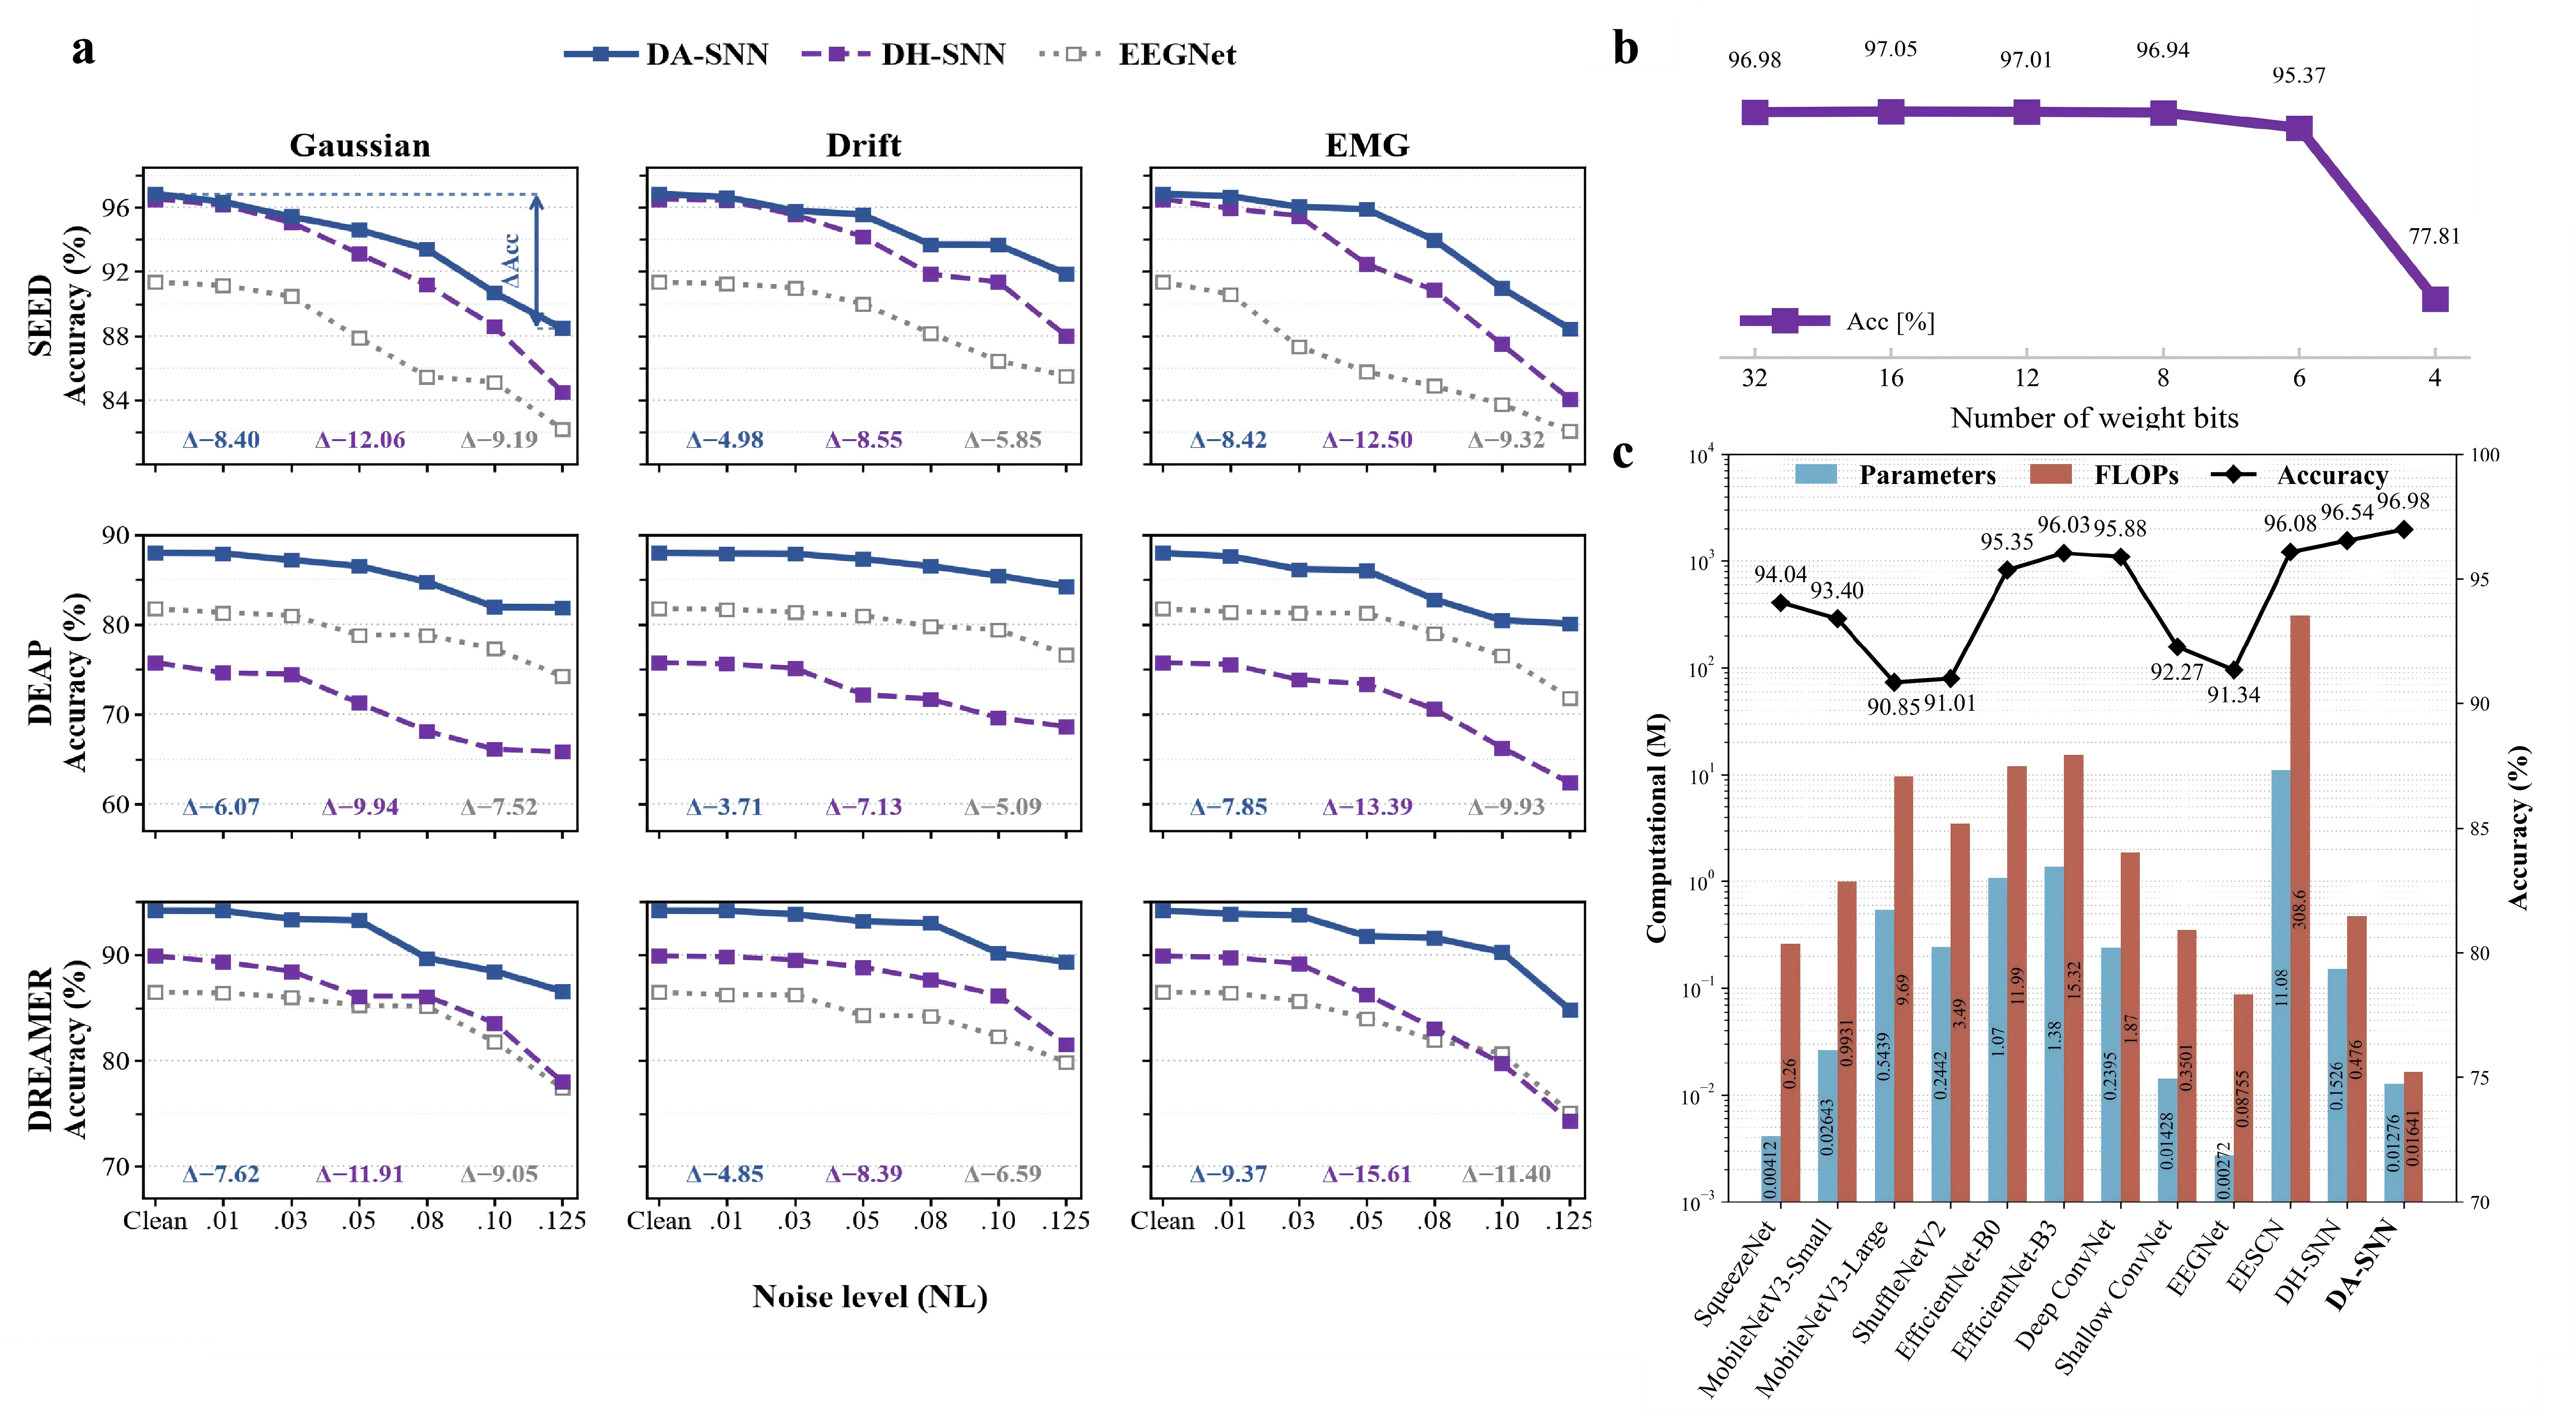
\includegraphics[width=0.95\textwidth]{figures/robustness_quantization_comparison.png}
\caption{
\textbf{Sensitivity to controlled EEG perturbations, weight quantization, and model complexity.}
\textbf{(a)} Single-seed accuracy of DA-SNN, DH-SNN, and EEGNet on SEED, DEAP, and DREAMER under Gaussian noise, low-frequency drift, and electromyographic (EMG)-like transient bursts. Perturbations were added to time-domain EEG samples before PSE extraction, spatial mapping, and LDS smoothing. Relative noise level (NL) denotes the ratio of the perturbation standard deviation to the clean signal standard deviation within each channel; Clean denotes NL$=0$. Endpoint annotations report $\Delta\mathrm{Acc}=\mathrm{Acc}_{\mathrm{NL}=0.125}-\mathrm{Acc}_{\mathrm{Clean}}$ in percentage points.
\textbf{(b)} SEED accuracy in a weight-bit-width sweep from 32 to 4 bits using quantization-aware training.
\textbf{(c)} Performance comparison of DA-SNN with representative lightweight models. FLOPs and parameter counts are normalized.
}
\label{fig:robust_quant_comparison}
\end{figure*}
{\small\noindent\textbf{Alt text:} A three-panel deployment-oriented evaluation. Panel (a) compares DA-SNN, DH-SNN, and EEGNet accuracy across clean EEG and increasing Gaussian, low-frequency-drift, and EMG-like perturbation levels on SEED, DEAP, and DREAMER. Panel (b) shows SEED accuracy across weight precisions from 32 to 4 bits. Panel (c) compares normalized accuracy, operation count, and parameter count for DA-SNN and representative lightweight models.\par}

\begin{table}[b]
\caption{Efficiency of comparison classifiers at the model level on Raspberry Pi~5. Operation counts use thousands of operations; MACs, multiply-accumulate operations. Memory values are reported in KB. FP32, 32-bit floating point; INT8, 8-bit integer. Integer inference is summarized by MACs, so the INT8 FLOPs entry is blank. FPGA results are reported separately.}
\label{tab:efficiency}

\setlength{\tabcolsep}{3pt}
\renewcommand{\arraystretch}{1.3}
\scriptsize

\sisetup{
  table-number-alignment=center,
  parse-numbers=true,
  detect-weight=true
}
\resizebox{\columnwidth}{!}{%
\begin{tabular}{@{}l
S[table-format=5.2]
S[table-format=6.2]
S[table-format=6.2]
S[table-format=5.2]
S[table-format=4.2]
S[table-format=3.2]@{}}
\toprule
Model
& {Params (K)}
& {FLOPs (K)}
& {MACs (K)}
& {\makecell{Parameter\\storage (KB)}}
& {\makecell{Runtime\\memory (KB)}}
& {Power (mW)} \\
\midrule

SqueezeNet        &   4.12 & 259.97 & 129.98 &  16.09 &  50.43 & 368.33 \\
MobileNetV3-Small &  26.43 & 993.12 & 496.56 & 103.23 & 392.44 & 458.33 \\
MobileNetV3-Large & 543.90 & 9690.00 & 4850.00 & 2119.68 & 3614.72 & 546.35 \\
ShuffleNetV2      & 244.22 & 3490.00 & 1740.00 & 953.98 & 1413.12 & 426.85 \\
EfficientNet-B0   & 1070.00 & 11990.00 & 6000.00 & 4198.40 & 5406.72 & 437.84 \\
EfficientNet-B3   & 1380.00 & 15320.00 & 7660.00 & 5396.48 & 7096.32 & 524.62 \\
Deep ConvNet      & 239.48 & 1870.00 & 936.20 & 935.46 & 995.98 & 435.53 \\
Shallow ConvNet   &  14.28 & 350.08 & 175.04 &  55.79 &  85.07 & 258.37 \\
EEGNet            &   2.72 &  87.55 &  43.78 &  10.64 &  41.04 & 334.86 \\
EESCN             & 11080.00 & 308590.00 & 154290.00 & 43284.48 & 225.12 & 776.79 \\
DH-SNN            & 152.58 & 476.00 & 235.96 & 587.01 & 260.89 & 236.49 \\

\midrule
\bfseries DA-SNN (FP32)
 & 12.76
 & 32.47
 & 16.23
 & 49.83
 & 51.27
 & 236.68 \\

\bfseries DA-SNN (INT8)
 & 12.76
 & {}
 & 16.23
 & 12.50
 & 13.68
 & 184.14 \\
\bottomrule
\end{tabular}%
} 
\end{table}


\begin{figure*}[t]
\centering
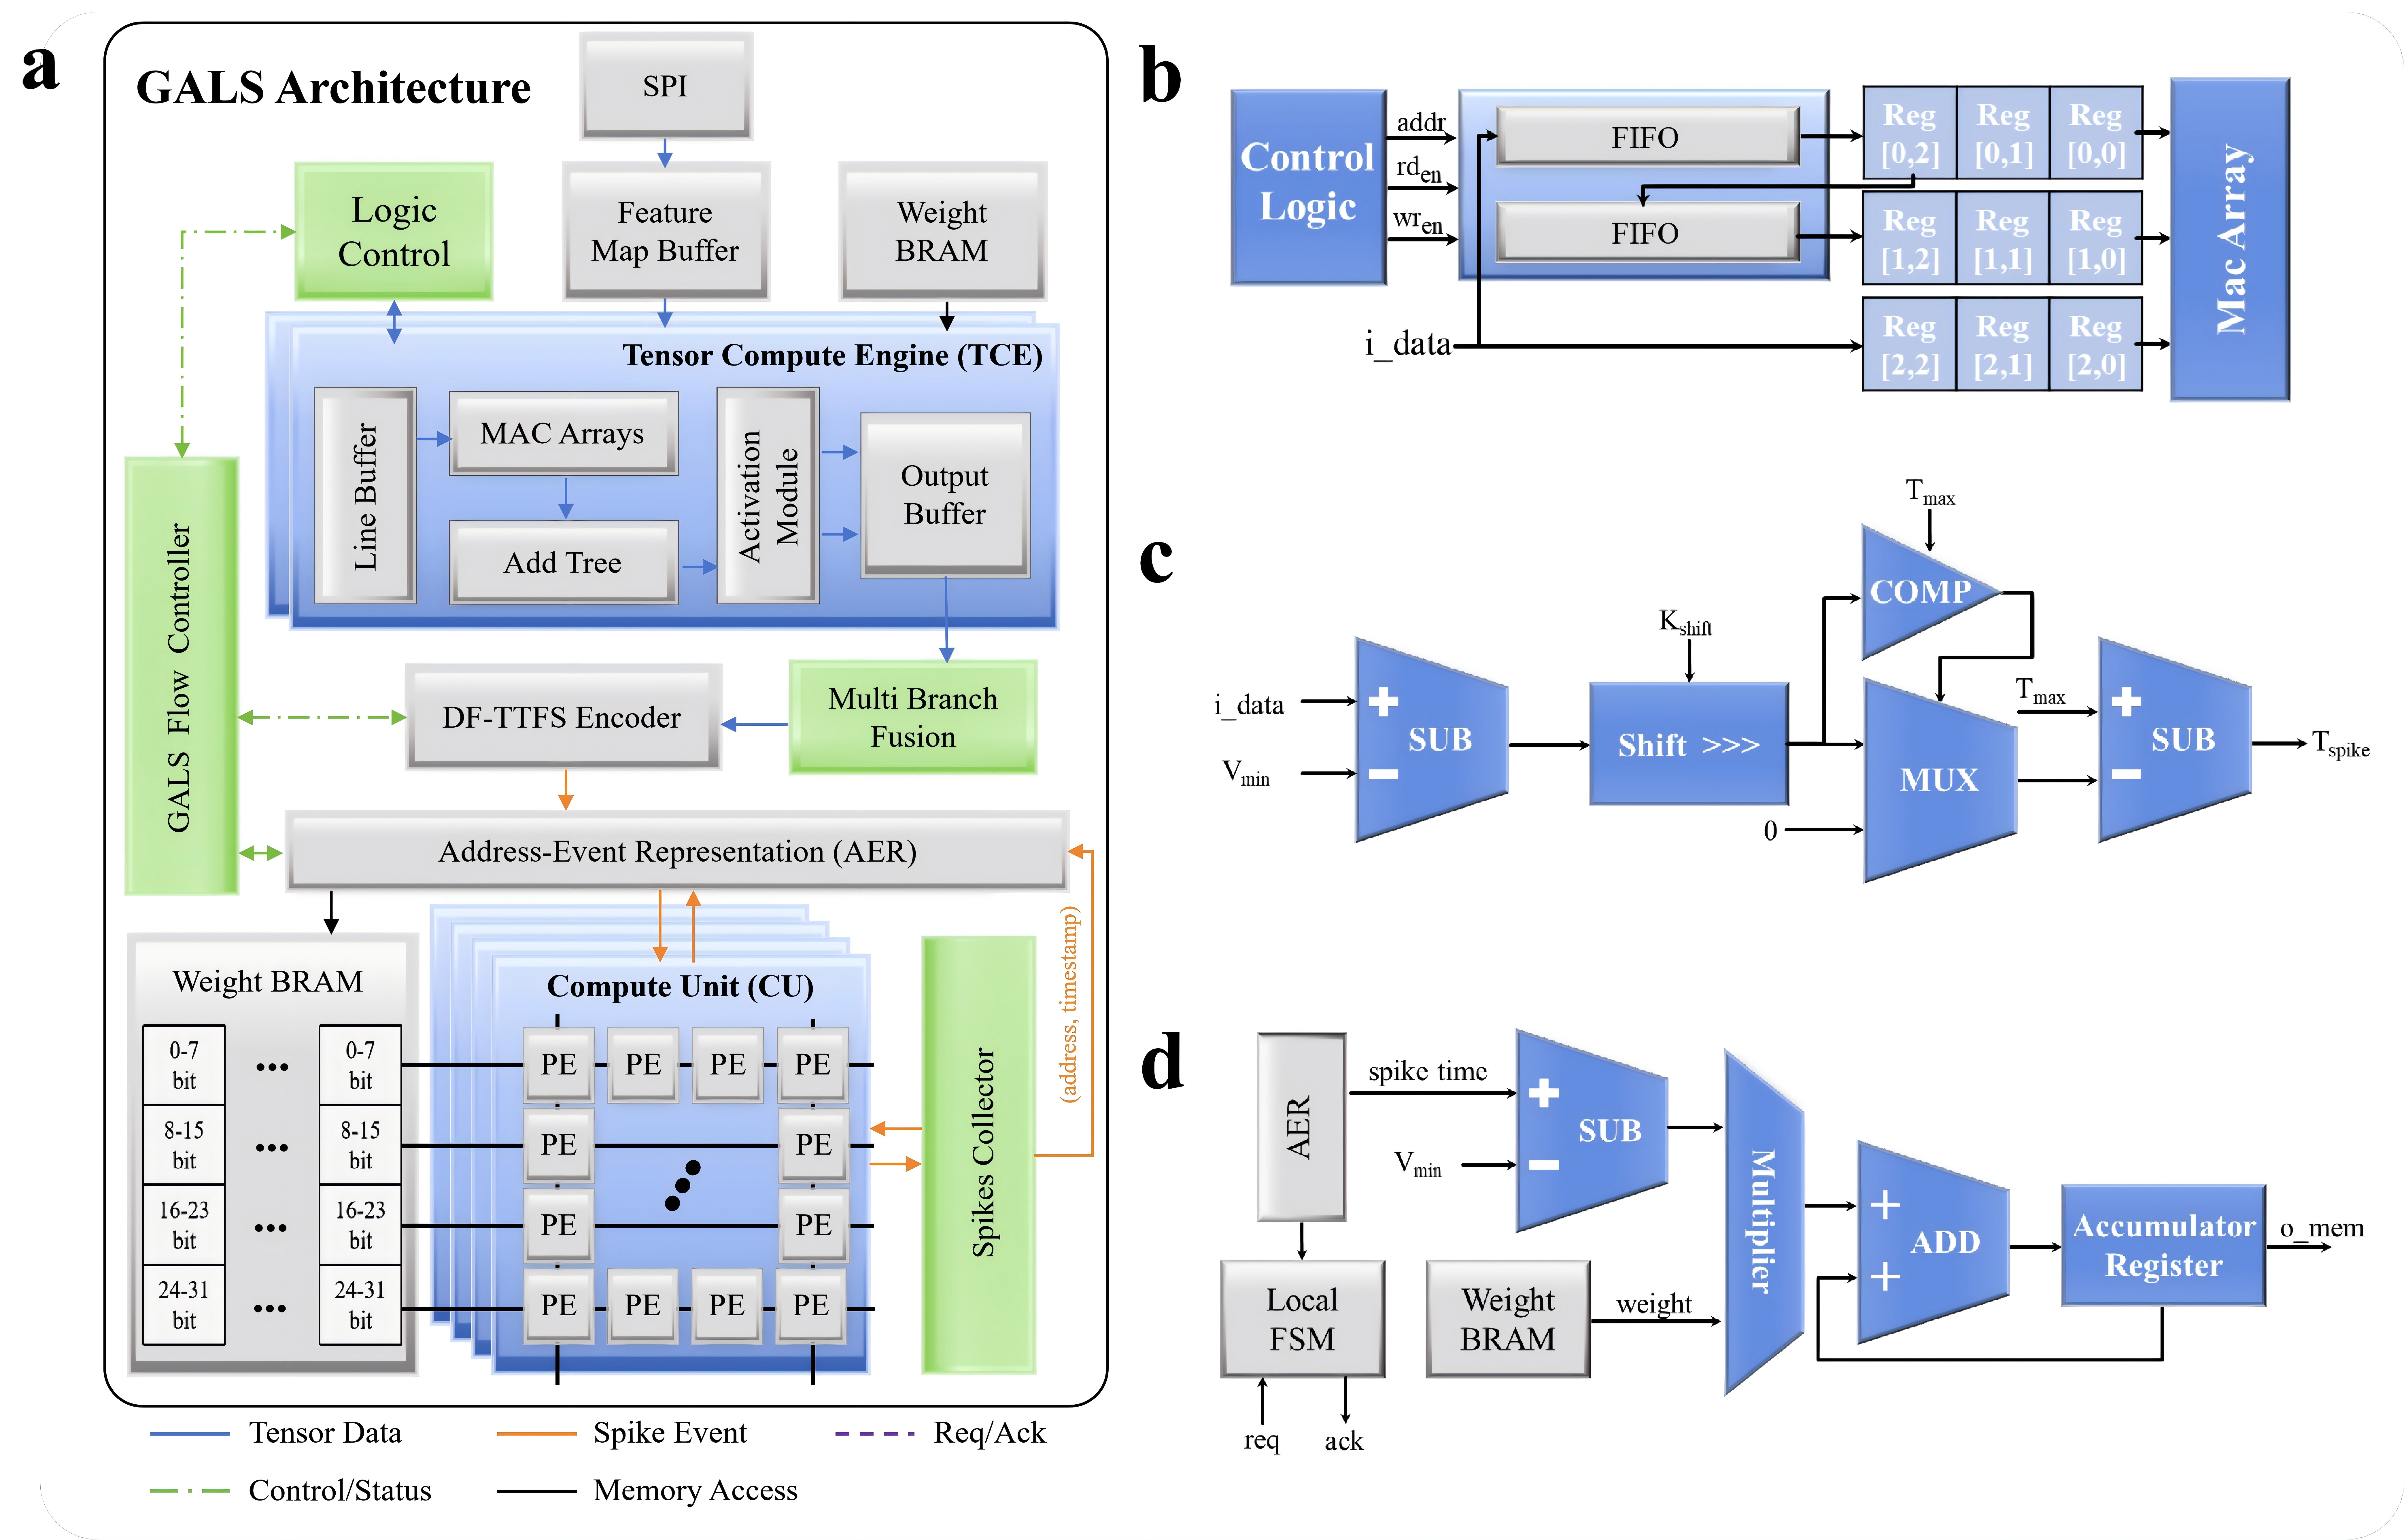
\includegraphics[width=\textwidth]{figures/hardoverview.png}
\caption{\textbf{Hardware architecture and main components of the proposed accelerator.}
(a) Organization of the globally asynchronous, locally synchronous (GALS) accelerator. Blue solid lines trace tensor data from the streaming INT8 tensor compute engine (TCE) to the division-free time-to-first-spike (DF-TTFS) encoder. Orange solid lines trace address-event representation (AER) spike events through the compute unit and processing element (CU/PE) arrays. Each event carries an address and timestamp, and hidden layer events enter the recirculation path. Purple dashed lines denote request/acknowledgment (Req/Ack) handshaking, green dash-dotted lines denote control and status, and thin black lines denote memory access. The tensor pipeline through DF-TTFS belongs to the local \texttt{clk\_TCE} island. The weight memory, CU/PE arrays, and spike collector belong to the independent \texttt{clk\_SNN} island, with the AER block forming the composite clock domain boundary.
(b) A shift register line buffer that continuously reconstructs sliding windows for pipelined convolution.
(c) Hardware implementation of the DF-TTFS encoder using shift based normalization and valid event detection to produce AER spikes.
(d) Microarchitecture of the event-driven PE, showing integration of membrane potentials with time modulation and local clock enable control. The GALS Flow Controller coordinates start, enable, completion, and layer or array state. It carries only control and status signals, while each island retains its local clock.}
\label{fig:hardoverview}
\end{figure*}
{\small\noindent\textbf{Alt text:} A hardware diagram with four panels. Panel (a) traces dense INT8 tensor data through the \texttt{clk\_TCE} island to DF-TTFS conversion. Address and timestamp events then cross a Req/Ack AER boundary into the independent \texttt{clk\_SNN} island. Events drive CU/PE computation, hidden layer events recirculate through the spike collector and AER path, and final membrane potentials pass to a decision unit. Panels (b)--(d) detail the line buffer, encoder, and event-driven PE.\par}

\subsection{Sensitivity to Controlled EEG Perturbations and Quantization}

We assessed sensitivity to controlled signal corruption on SEED, DEAP, and DREAMER using additive Gaussian noise, low frequency drift, and EMG-like transient bursts (Fig.~\ref{fig:robust_quant_comparison}a). Each perturbation was applied to time domain EEG samples after signal conditioning and segmentation for each dataset. The perturbations preceded PSE extraction, spatial mapping, and LDS smoothing. The relative noise level was defined per channel as $\mathrm{NL}=\sigma_{\mathrm{noise}}/\sigma_{\mathrm{signal}}$ and varied over $\{0.01,0.03,0.05,0.08,0.10,0.125\}$. For each noisy feature bundle, DA-SNN, DH-SNN, and EEGNet used the same random window-level 80/20 protocol and random seed for training, selection, and evaluation. At NL$=0.125$, the accuracy decrease from clean data ranged from 3.71 to 9.37 percentage points for DA-SNN across the nine dataset--perturbation combinations. The corresponding ranges were 7.13--15.61 points for DH-SNN and 5.09--11.40 points for EEGNet. DA-SNN showed the smallest endpoint decrease in all nine comparisons. These single seed experiments with training matched to each noise condition provide descriptive evidence of lower sensitivity under controlled corruption. Statistical significance and robustness without retraining in wearable recordings remain outside their scope.

We further examined sensitivity to weight quantization by reducing weight precision from 32-bit floating point to 16, 12, 8, 6, and 4 bits using quantization-aware training (Fig.~\ref{fig:robust_quant_comparison}b). Accuracy changed from 96.98\% at 32 bits to 96.94\% at 8 bits, a decrease of 0.04 percentage points. The 6-bit configuration achieved 95.37\%, whereas accuracy fell to 77.81\% at 4 bits. These results support the selected 8-bit weight configuration under the evaluated SEED protocol. Performance below 8 bits varied with precision. The deployed integer model uses signed INT8 weights and unsigned 8-bit nonnegative activations, as detailed in the Supplementary Information.

\subsection{Computational Efficiency and Energy Consumption}

We analyze model scale, inference cost, memory footprint, and measured power on a Raspberry Pi~5. DA-SNN contains 12.76~K parameters (Table~\ref{tab:efficiency}), fewer than the MobileNetV3-Large and EfficientNet-B0 implementations evaluated under the same setting.

With TTFS encoding, each neuron emits at most one spike per inference cycle, and the measured average firing rate is 35.26\%. Under sparse execution, the profiler estimates 16.41~K floating-point operations and 8.21~K multiply-accumulate operations, compared with dense upper bounds of 32.47~K and 16.23~K, respectively. For the 32-bit floating-point model, parameter storage and runtime memory are 49.83~KB and 51.27~KB. INT8 quantization reduces these values to 12.50~KB and 13.68~KB, with a measured Raspberry Pi~5 energy of 261.21~$\mu$J per inference. These measurements characterize the model-level accuracy--cost trade-off shown in Fig.~\ref{fig:robust_quant_comparison}c.



\subsection{Hardware Implementation}

We implemented a heterogeneous accelerator for edge EEG inference. The design combines 8-bit integer quantization for each tensor with event-driven execution in a globally asynchronous, locally synchronous (GALS) organization (Supplementary Note~S2.4). It integrates a low bit width datapath, a reconfigurable tensor streaming subsystem, and a bundled-data interface between two local clock islands.

The combined streaming and event processing pipeline establishes the accelerator data flow (Fig.~\ref{fig:hardoverview}a). Multichannel data first stream into the on-chip input buffer through a serial peripheral interface (SPI). The reconfigurable tensor compute engine (TCE), multibranch fusion path, and DF-TTFS encoder operate in the local \texttt{clk\_TCE} island. A line buffer based on shift registers reconstructs sliding windows for pipelined convolution (Fig.~\ref{fig:hardoverview}b), after which the fused INT8 tensor enters DF-TTFS. The encoder forms the representation boundary by converting the dense tensor into sparse AER events. Each event carries an address and timestamp \cite{AER}. The AER block forms a composite interface. Its sending side generates the event and request, while clock domain crossing (CDC) logic transfers the handshake. Routing on the \texttt{clk\_SNN} side then delivers the event to the weight memory and CU/PE arrays.

Each event crossing between domains uses a bundled-data four-phase handshake \cite{ref72}. The sender first stabilizes the address and timestamp bus and asserts Req. After the \texttt{clk\_SNN} island observes the synchronized Req, the required array processes the event and asserts Ack on completion. The sender then deasserts Req, followed by Ack at the receiver, before releasing or replacing the payload. This stall behavior supplies backpressure through the handshake and uses no dual-clock first-in, first-out (FIFO) event buffer. The GALS Flow Controller coordinates start, enable, completion, and layer or array state across the pipeline. Payload transfer remains in the AER interface, and each island retains its local execution clock. The detailed CDC sequence is provided in the Supplementary Information.

The accelerator uses a streaming reconfigurable TCE that time-multiplexes shared compute resources across the convolution variants. The TCE consists of control logic, a shared multiply-accumulate array, an adder tree, and a multifunction activation unit. The datapath is reconfigured when the workload enters the multibranch gating stage. At this stage, concurrent access by the main branch, channel gate, and spatial gate exceeds the port limit of standard dual-port block RAMs (BRAMs). A multibank buffer therefore supports one write stream and three read streams per pipeline stage. The output stage also fuses batch normalization, quantization, and activation within one datapath to reduce pipeline depth.

The division-free encoding module forms the tensor-to-event boundary within the \texttt{clk\_TCE} island. During quantization-aware training, the scaling factor $S_p$ is constrained to a power of two ($S_p=2^k$). A barrel shifter can then replace floating-point division with a right shift. As illustrated in Fig.~\ref{fig:hardoverview}c, shift based normalization and valid event detection generate address and timestamp events directly from INT8 features. The resulting combinational datapath computes spike latencies within a single local clock cycle.

To address frequent weight access and sparse neural activity in SNN inference, the \texttt{clk\_SNN} island uses an array architecture centered on memory. Placing weight storage beside computation alleviates bandwidth pressure and reduces data movement. The compute fabric contains 16 independent SNN arrays, each with four event-driven processing elements. The microarchitecture of each PE, shown in Fig.~\ref{fig:hardoverview}d, integrates the membrane potential with time modulation under a local finite state machine and register clock enable. The AER interface broadcasts events to active arrays. Hidden layer events follow the CU/PE--spike collector--AER--CU/PE recirculation path as subsequent layers reuse the hardware over time. A separate comparator tree classifies the final layer from its 32-bit membrane potentials and outputs the argmax class label.

To evaluate hardware deployment, we implemented the INT8 model on a Xilinx Zynq-7020 system-on-chip (SoC). The accelerator resides in the programmable logic and operates at 100~MHz with a 1.0~V core supply voltage. Look-up table (LUT) and flip-flop (FF) utilization are 20.34\% and 7.67\%, respectively (Supplementary Table~S9). For one accelerator inference from a preprocessed tensor, the GALS implementation achieves 18~$\mu$s latency. It consumes 40~mW of dynamic power and 108~mW of static power, giving 148~mW total power and 2.66~$\mu$J total energy per inference. This accelerator boundary begins after PSE and LDS preprocessing.

We additionally implemented a matched synchronous version of the same INT8 DA-SNN on the same FPGA using the same input tensor and clock enable policy. Relative to this matched implementation, GALS adds 172 LUTs and 139 FFs and increases latency from 16.5 to 18~$\mu$s. Total energy decreases from 3.35 to 2.66~$\mu$J per inference. This comparison isolates the effect of GALS within the implementation.

As an FPGA baseline across models, we also implemented EEGNet on the Zynq-7020 platform (Supplementary Table~S11). Compared with EEGNet, the GALS DA-SNN uses more logic and memory resources and slightly higher total power (148 versus 138~mW). Its inference latency decreases from 0.772~ms to 18~$\mu$s, and total energy decreases from 106.536 to 2.66~$\mu$J per inference. This deployment comparison covers differences in both model architecture and clock target. The matched synchronous comparison above isolates the effect of GALS.


\section{DISCUSSION}
Consistent with the integrated perspective of neuromorphic computing \cite{ref71}, the results suggest that the framework benefits from coordination among its components. Across five EEG emotion recognition benchmarks, the framework maintains strong performance under different emotion categories and subject conditions. In controlled perturbation tests with a single seed, DA-SNN showed a smaller endpoint accuracy decrease than DH-SNN and EEGNet in all nine dataset--perturbation combinations. The 8-bit weight setting also differed from its 32-bit counterpart by only 0.04 percentage points. These findings support deployment focused evaluation under the tested conditions; uncontrolled wearable artifacts require separate study.

The ablation and diagnostic results clarify the distinct, complementary roles of the main algorithmic components. Removing DSGM reduces mean accuracy on all three ablation datasets, with a magnitude that varies by dataset. DF-TTFS converts dense features into sparse spike times through power-of-two scaling. Conventional min--max normalization produces mixed accuracy differences across datasets, placing the contribution of DF-TTFS in removing floating-point division from the hardware path. For ATSNN, the training trajectory shows that the two hidden layers learn different temporal ranges and settle during late training. Fixed temporal windows also yield lower mean accuracy on all three datasets. Together, these results associate the components with feature selection, hardware oriented event encoding, and temporal adaptation.

The efficiency mechanisms act at three levels. First, the measured 35.26\% average firing rate reflects event sparsity in the model, reducing AER transfers, weight reads, and membrane potential updates. Second, event-triggered execution and data movement activate routing, memory access, and CU/PE computation only for valid events. Third, local register clock enables hold completed or inactive datapaths in an idle state. This control reduces dynamic switching in clocked states and datapaths but leaves static power unchanged. INT8 quantization separately compresses parameter storage and runtime memory by 4$\times$, reducing them to 12.50~KB and 13.68~KB, respectively. The GALS boundary also consumes resources and adds functional latency. Top level hierarchical synthesis resolves these contributions for event filtering, AER routing, address decoding, Req/Ack synchronizers, handshake state machines, and clock enable control. The Supplementary Information reports these values, while component power remains aggregated within the measured accelerator power.

The two FPGA baselines answer different questions and remain separate from the Raspberry Pi comparison in Table~\ref{tab:efficiency}, which evaluates models on a general purpose platform. The matched synchronous DA-SNN isolates the GALS implementation trade-off. GALS incurs modest logic and latency overhead while reducing total energy per inference by 20.6\%. The independently deployed EEGNet provides a reference across models. DA-SNN requires more FPGA resources and slightly higher total power, but its shorter latency yields 97.5\% lower total energy per inference. These comparisons quantify implementation and deployment trade-offs under the measured conditions. Causal attribution to GALS is limited to the matched comparison of the same DA-SNN.

The present study evaluates a fixed parameter inference architecture. The subject-independent protocols assess a fixed model across held-out subjects, leaving longitudinal changes and personalization during prolonged use for future evaluation. The single seed perturbation tests similarly address controlled synthetic corruption with training matched to each noise condition. Naturally occurring motion, electromyographic (EMG), electrooculographic (EOG), electrode contact, impedance, and sweat artifacts require recordings from wearable use. The reported 18~$\mu$s latency applies to accelerator inference from one preprocessed tensor. The 12.50~KB parameter storage and 13.68~KB runtime memory describe the model footprint. PSE and LDS were characterized as standalone FPGA kernels. EEG acquisition, the sensor front end, communication, and battery operation remain to be integrated. Future work should measure acquisition to decision latency, total memory, energy, and stability during continuous operation. It should also evaluate session calibration or selective parameter adaptation, including their storage, update logic, and energy costs. An application-specific integrated circuit (ASIC) could then define the area and power envelope beyond the present FPGA prototype.

\section{CONCLUSION}
This work presents an integrated neuromorphic design for low power wearable EEG emotion recognition. The framework combines sparse temporal encoding, spiking inference, and GALS hardware execution while maintaining strong recognition performance across five benchmark datasets. Controlled perturbation tests show lower endpoint sensitivity than two matched baselines across the evaluated dataset--noise combinations. On SEED, the 8-bit weight setting retains accuracy within 0.04 percentage points of the 32-bit result. Within these experimental boundaries, the system processes affective features derived from EEG as sparse events with limited loss of recognition performance. It therefore provides an alternative to synchronous dense computation for deployment.

Efficiency gains occur at both the model and hardware levels. The INT8 network requires 12.50~KB of parameter storage and 13.68~KB of runtime memory. It consumes 261.21~$\mu$J per inference on Raspberry Pi~5. Within the accelerator inference boundary, the GALS FPGA implementation achieves 18~$\mu$s latency, 40~mW dynamic power, and 2.66~$\mu$J total energy per inference. The matched synchronous implementation requires 3.35~$\mu$J, and the independently deployed FPGA EEGNet requires 106.536~$\mu$J. These results map algorithmic sparsity to event-triggered hardware activity under the evaluated conditions and support accelerator inference with low power from preprocessed EEG tensors. The energy breakdown excludes PSE and LDS preprocessing and reports interface power only within the accelerator total. Future systems integrating sensors should evaluate complete operation, natural artifacts, and online adaptation.

\section{METHODS}
Main Table~\ref{tab:overall_15models} uses a subject-dependent random window-level 80/20 evaluation protocol. Complementary subject-independent evaluations and full details of dataset composition, preprocessing, data splitting, model selection, and statistical aggregation are provided in the online Supplementary Information.

\section{DATA AND CODE AVAILABILITY}
The source code is available at \url{https://github.com/BhealthE6315/DA-SNN}.

\section{FUNDING}
This work was supported by the National Natural Science Foundation of China (No. 62227807).

\bibliographystyle{nsr}
\bibliography{nsr_sample}
\end{document}
